\documentclass[hyperref={bookmarks=false},aspectratio=169]{beamer}
\usepackage{hyperref,ragged2e,amsmath,amssymb,url,bm}
\usepackage{graphicx,booktabs,array}
\newcolumntype{P}[1]{>{\RaggedRight\arraybackslash}p{#1}}
\usepackage{tikz}
\usetikzlibrary{arrows.meta,positioning,calc,shapes.geometric,decorations.pathreplacing,matrix}
\usepackage{pgfplots}\pgfplotsset{compat=1.18}
\graphicspath{{crops/}}
\usetheme{Goettingen}
\definecolor{azulp}{RGB}{16,42,86}
\definecolor{azulo}{RGB}{8,20,45}
\definecolor{celeste}{RGB}{201,160,48}
\definecolor{azulcl}{RGB}{250,244,228}
\definecolor{grisaz}{RGB}{60,70,92}
\setbeamercolor{structure}{fg=azulp}
\setbeamertemplate{sidebar canvas right}[vertical shading][top=azulp!92!black,bottom=azulo]
\setbeamercolor{title in sidebar}{fg=celeste}
\setbeamercolor{author in sidebar}{fg=azulcl}
\setbeamercolor{section in sidebar}{fg=celeste}
\setbeamercolor{section in sidebar shaded}{fg=azulcl!55!azulp}
\setbeamercolor{subsection in sidebar}{fg=azulcl}
\setbeamercolor{subsection in sidebar shaded}{fg=azulcl!55!azulp}
\let\raggedright\justifying
\setbeamertemplate{background canvas}{
\includegraphics[width=\paperwidth,height=\paperheight]{papiro_crema.jpg}}
\setbeamercolor{normal text}{fg=azulo}
\setbeamercolor{frametitle}{fg=azulp}
\setbeamerfont{frametitle}{series=\bfseries}
\setbeamertemplate{section in toc shaded}{\leavevmode{\color{grisaz!85!black}\inserttocsection}\par}
\setbeamercolor{title}{fg=azulp}
\setbeamercolor{subtitle}{fg=grisaz}
\setbeamercolor{item projected}{bg=azulp,fg=azulcl}
\setbeamertemplate{itemize item}{\small\textcolor{celeste!80!azulp}{$\blacktriangleright$}}
\setbeamertemplate{navigation symbols}{}
\usepackage[bidi=default]{babel}
\babelprovide[import,main]{spanish}
\babelprovide[import]{hebrew}
\babelprovide[import]{ancientgreek}
\babelfont[hebrew]{sf}[Path=fonts/, BoldFont=NotoHebrewSans-700.ttf]{NotoHebrewSans-400.ttf}
\babelfont[hebrew]{rm}[Path=fonts/, BoldFont=NotoHebrewSans-700.ttf]{NotoHebrewSans-400.ttf}
\babelfont[ancientgreek]{sf}[Path=fonts/]{GFSPorson.otf}
\babelfont[ancientgreek]{rm}[Path=fonts/]{GFSPorson.otf}
\newcommand{\heb}[1]{\mbox{\foreignlanguage{hebrew}{#1}}}
\newcommand{\grc}[1]{\foreignlanguage{ancientgreek}{#1}}
\usepackage[most]{tcolorbox}
\newtcolorbox{cita}[1][]{enhanced, colback=azulcl, colframe=celeste,
  boxrule=0pt, leftrule=2.5pt, arc=0pt, left=6pt, right=6pt, top=4pt, bottom=4pt,
  before skip=4pt, after skip=6pt, fontupper=\small\itshape, #1}
\newcommand{\fuente}[1]{\par\hfill{\upshape\bfseries\footnotesize\textcolor{azulp}{#1}}}
\newcommand{\imagen}[3][0.80]{%
  \centering\includegraphics[height=#1\textheight,width=\linewidth,keepaspectratio]{#2}\par\vspace{2pt}
  {\fontsize{5}{6}\selectfont\color{grisaz}{\raggedleft\textit{Nota.} #3\par}}}
\makeatletter
\newcommand{\fotolado}[2]{%
  \begin{tikzpicture}[remember picture,overlay]
    \node[anchor=north east,inner sep=0pt] (foto) at ([xshift=-\beamer@sidebarwidth]current page.north east)
      {\includegraphics[height=\paperheight]{#1}};
  \end{tikzpicture}}
\makeatother
\newcommand{\refapa}[1]{\par\hangindent=1.2em\hangafter=1\noindent #1\par\vspace{3pt}}
\usepackage{xurl}\urlstyle{same}
\newcommand{\destacar}[1]{\textbf{\textcolor{azulp}{#1}}}
\tikzset{caja/.style={draw=azulp,line width=0.8pt,fill=azulcl,fill opacity=0.88,text opacity=1,rounded corners=3pt,inner sep=5pt,font=\scriptsize}}

\newcommand{\SENOR}{SEÑOR}
\setbeamertemplate{frametitle}{\vspace*{3pt}{\usebeamerfont{frametitle}\usebeamercolor[fg]{frametitle}\insertframetitle}\par\vspace{1pt}{\color{celeste}\rule{2.4cm}{1.6pt}}}
\setbeamertemplate{itemize item}{\small\textcolor{celeste}{$\blacktriangleright$}}
\newcolumntype{P}[1]{>{\RaggedRight\arraybackslash}p{#1}}
\renewcommand{\arraystretch}{1.3}
\title[Atributos de Dios]{\bfseries{Conociendo al Dios de la Biblia}}
\subtitle{Los atributos de Dios — Introducción}
\author{}\institute{}\date{}
\titlegraphic{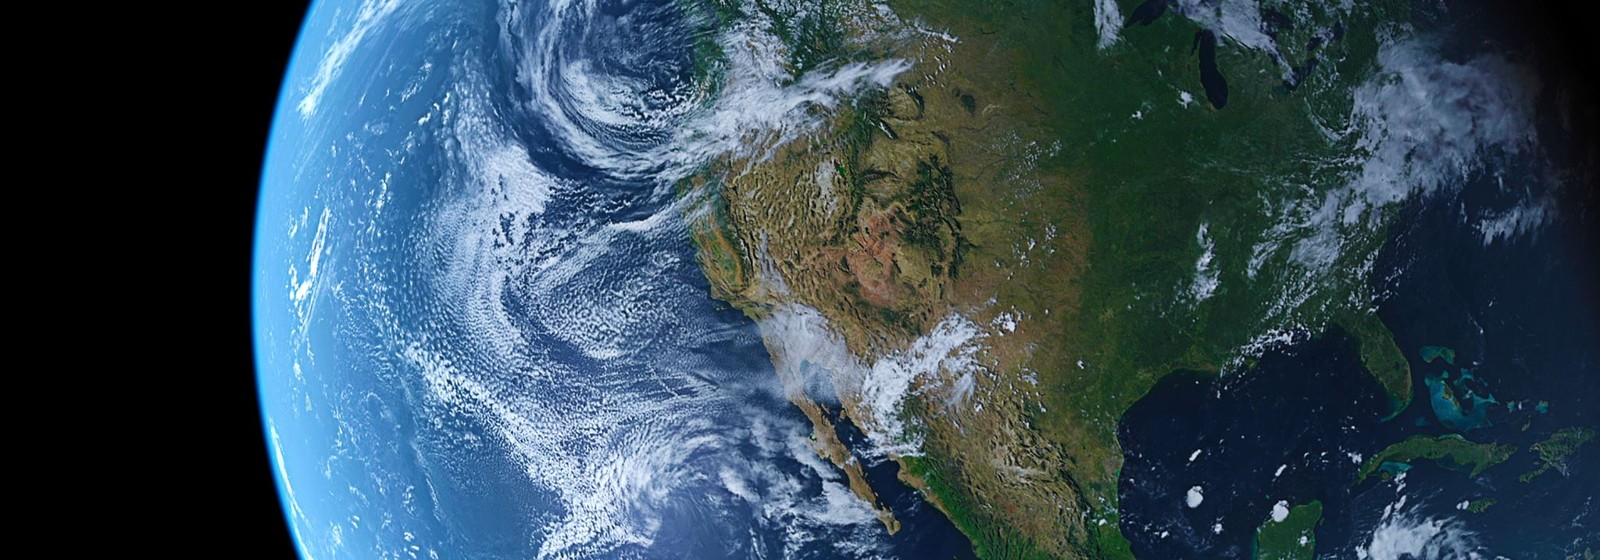
\includegraphics[width=0.85\linewidth,height=0.40\textheight,keepaspectratio]{portada.jpg}}
\AtBeginSection[]{\ifnum\value{section}>1\begin{frame}\frametitle{Contenidos}\tableofcontents[currentsection]\end{frame}\fi}
\begin{document}
\frame{\titlepage}
\begin{frame}\frametitle{Contenidos}\tableofcontents\end{frame}

% =====================================================================
\section{Introducción}
% =====================================================================
\begin{frame}{El verso que lo une todo}
\fotolado{p_tierra_noche.jpg}{}
\begin{columns}[c,onlytextwidth]
\begin{column}{0.57\textwidth}
\begin{cita}Así dijo el \SENOR: No se alabe el sabio en su sabiduría, ni en su valentía se alabe el valiente, ni el rico se alabe en sus riquezas.\\[4pt]
Mas alábese en esto el que se hubiere de alabar: en entenderme y conocerme, que yo soy el \SENOR, que hago misericordia, juicio y justicia en la tierra; porque estas cosas quiero, dice el \SENOR.\fuente{(Jeremías 9:23–24, RVR1960)}\end{cita}
\end{column}
\begin{column}{0.41\textwidth}\end{column}
\end{columns}
\end{frame}

\begin{frame}{Tres glorias falsas, una verdadera}
\centering
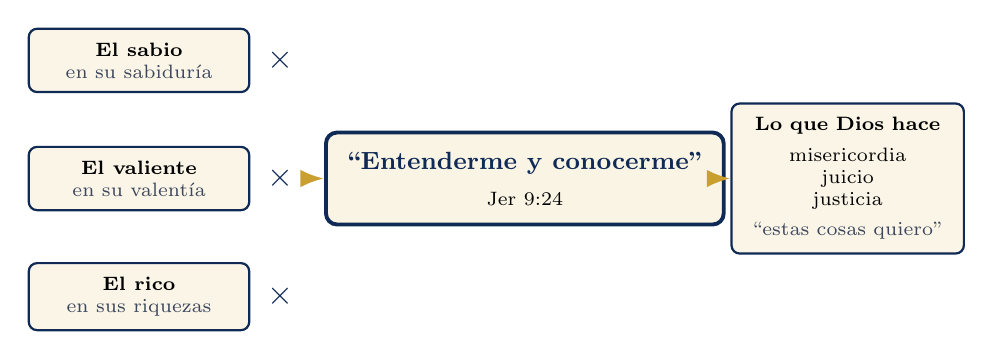
\begin{tikzpicture}[font=\scriptsize]
 \foreach \y/\p/\c in {1.5/El sabio/{en su sabiduría},0/El valiente/{en su valentía},-1.5/El rico/{en sus riquezas}}{
   \node[caja,minimum width=2.8cm,align=center] at (0,\y) {\textbf{\p}\\{\color{grisaz}\c}};
   \node[text=azulp,font=\large\bfseries] at (1.8,\y) {$\times$};}
 \node[draw=azulp,line width=1.4pt,fill=azulcl,rounded corners=4pt,align=center,inner sep=7pt,font=\small] (v) at (4.9,0)
   {\textbf{\textcolor{azulp}{“Entenderme y conocerme”}}\\[2pt]{\scriptsize Jer 9:24}};
 \draw[-{Latex[length=3mm]},line width=1.2pt,celeste] (2.1,0) -- (v.west);
 \node[caja,align=center,text width=2.6cm] (q) at (9.0,0) {\textbf{Lo que Dios hace}\\[3pt]misericordia\\juicio\\justicia\\[3pt]{\color{grisaz}“estas cosas quiero”}};
 \draw[-{Latex[length=3mm]},line width=1.2pt,celeste] (v.east) -- (q.west);
\end{tikzpicture}
\vspace{8pt}

\small Dios no prohíbe gloriarse: cambia el \destacar{objeto} de la gloria. La única gloria que permanece es conocerle.
\end{frame}

\begin{frame}{Conocer por experiencia}
\begin{tcolorbox}[colback=azulcl,colframe=azulp,boxrule=1pt,arc=3pt,fontupper=\small]
\textbf{Barry J. Marshall} (1951– ), médico australiano y Premio Nobel de Medicina (2005), estudiaba las enfermedades gástricas. En 1984, para demostrar su hipótesis, \destacar{experimentó en su propio cuerpo} la bacteria \emph{Helicobacter pylori}, desarrollando gastritis. Esta experiencia confirmó su teoría y transformó la medicina digestiva mundial (Marshall et al., 1985).
\end{tcolorbox}
\vspace{4pt}
\small Marshall no solo \emph{sabía} de la bacteria: la \destacar{conoció en su cuerpo}. Así es el conocimiento de Dios al que llama Jeremías.
\end{frame}

% =====================================================================
% =====================================================================
\begin{frame}{Entender a Dios}
\scriptsize
\begin{tabular}{@{}P{1.6cm} P{1.5cm} P{3.8cm} P{1.4cm} P{2.2cm}@{}}
\toprule
\textbf{Término en español} & \textbf{Transliteración} & \textbf{Definición clave} & \textbf{Enfoque} & \textbf{Vivencia práctica} \\ \midrule
\destacar{Entender a Dios} & \emph{haskél} & Comprender cómo Dios actúa en la historia del ser humano y en la vida de cada individuo, qué valora según su carácter santo y fiel, cómo gobierna soberanamente con justicia, misericordia y verdad. & Intelectual–práctico & Discernir la voluntad de Dios y vivir conforme a ella. \\ \bottomrule
\end{tabular}
\end{frame}

\begin{frame}{Conocer a Dios}
\scriptsize
\begin{tabular}{@{}P{1.6cm} P{1.5cm} P{3.8cm} P{1.4cm} P{2.2cm}@{}}
\toprule
\textbf{Término en español} & \textbf{Transliteración} & \textbf{Definición clave} & \textbf{Enfoque} & \textbf{Vivencia práctica} \\ \midrule
\destacar{Conocer a Dios} & \emph{ve-yadó‘a} & Vivir en relación personal, de pacto y experiencial con Él. & Relacional–pacto & Comunión real con Dios, fidelidad al pacto, vida delante de Él. \\ \bottomrule
\end{tabular}
\vspace{12pt}

\begin{columns}[c,onlytextwidth]
\begin{column}{0.48\textwidth}
\begin{tcolorbox}[colback=azulcl,colframe=azulp,boxrule=0.8pt,arc=3pt,fontupper=\small,halign=center]
\textbf{Entender}\\ la mente: cómo es y cómo actúa
\end{tcolorbox}
\end{column}
\begin{column}{0.48\textwidth}
\begin{tcolorbox}[colback=azulcl,colframe=azulp,boxrule=0.8pt,arc=3pt,fontupper=\small,halign=center]
\textbf{Conocer}\\ la relación: vivir con Él en pacto
\end{tcolorbox}
\end{column}
\end{columns}
\end{frame}

\begin{frame}{La Escritura sobre conocerle}
\tiny
\begin{tabular}{@{}P{1.2cm} P{4.9cm} P{4.9cm}@{}}
\toprule
 & \textbf{Reina-Valera 1960 (RVR60)} & \textbf{Nueva Versión Internacional (NVI)} \\ \midrule
Sal 91:14 & Por cuanto en mí ha puesto su amor, yo también lo libraré; le pondré en alto, por cuanto ha conocido mi nombre. & «Yo lo libraré, porque él se acoge a mí; lo protegeré, porque reconoce mi nombre». \\
Mt 11:27 & Todas las cosas me fueron entregadas por mi Padre; y nadie conoce al Hijo, sino el Padre, ni al Padre conoce alguno, sino el Hijo, y aquel a quien el Hijo lo quiera revelar. & Todas las cosas me han sido entregadas por mi Padre. Nadie conoce al Hijo sino el Padre, y nadie conoce al Padre sino el Hijo y aquel a quien el Hijo quiera revelarlo. \\
Jn 17:3 & Y esta es la vida eterna: que te conozcan a ti, el único Dios verdadero, y a Jesucristo, a quien has enviado. & Y esta es la vida eterna: que te conozcan a ti, el único Dios verdadero, y a Jesucristo, a quien tú has enviado. \\
1 Jn 5:20 & Pero sabemos que el Hijo de Dios ha venido, y nos ha dado entendimiento para conocer al que es verdadero… & También sabemos que el Hijo de Dios ha venido y nos ha dado entendimiento para que conozcamos al Dios verdadero… \\ \bottomrule
\end{tabular}
\end{frame}

\begin{frame}{Medios de revelación}
\scriptsize
\begin{tabular}{@{}P{2.3cm} P{3.0cm} P{3.0cm} P{2.4cm}@{}}
\toprule
\textbf{Medio de revelación} & \textbf{Qué revela de Dios} & \textbf{Idea clave} & \textbf{Referencias bíblicas} \\ \midrule
\destacar{Biblia (Palabra)} & Su carácter, voluntad y plan redentor & Revelación especial, clara y normativa & Sal 19:7–11 \\
\destacar{Naturaleza} & Su existencia, poder, gloria y sabiduría & Revelación general, universal & Sal 19:1–6; Ro 1:19–20 \\
\destacar{Seres vivos / experiencias de vida} & Su cuidado, bondad y gobierno continuo & Dios sostiene y gobierna la vida & Job 12:7–10; Sal 104 \\ \bottomrule
\end{tabular}
\end{frame}

% =====================================================================
\section[Definiciones generales]{Definiciones generales}
% =====================================================================
\begin{frame}{Definiciones generales}
\begin{tcolorbox}[colback=azulcl,colframe=azulp,boxrule=1pt,arc=3pt,fontupper=\small]
Un \destacar{atributo} es una perfección eterna que Dios revela de sí mismo en la Escritura y por la cual podemos conocerle.
\end{tcolorbox}
\begin{itemize}\small
\item Todos los atributos son \destacar{perfecciones eternas} de Dios.
\item Algunos expresan lo que Dios \emph{es}; otros, \emph{quién es}; y otros se fueron \destacar{revelando en su relación con el ser humano}.
\item Dios se dio a conocer proclamando su Nombre (Éx 33:18–19; 34:6–7).
\end{itemize}
\begin{cita}No se puede confiar, ni servir, ni adorar a un Dios desconocido.\fuente{(Pink, 2020, p. 4)}\end{cita}
\end{frame}

% =====================================================================
\section[Clasificación]{Clasificación de los atributos}
% =====================================================================
\newcommand{\clasif}[8]{%
\begin{frame}{#2}
\fotolado{#1}{}
\begin{columns}[t,onlytextwidth]
\begin{column}{0.57\textwidth}
\scriptsize
{\bfseries\color{celeste}PALABRA CLAVE: #3}\par\vspace{5pt}
\textbf{Definición breve:} #4\par\vspace{4pt}
\textbf{Rasgos centrales:} #5\par\vspace{4pt}
\textbf{Ejemplos:} #6\par\vspace{4pt}
\textbf{#7}\par\vspace{4pt}
{\color{grisaz}\textbf{Referencias bíblicas:} #8}
\end{column}
\begin{column}{0.41\textwidth}\end{column}
\end{columns}
\end{frame}}

\begin{frame}{Primera clasificación}
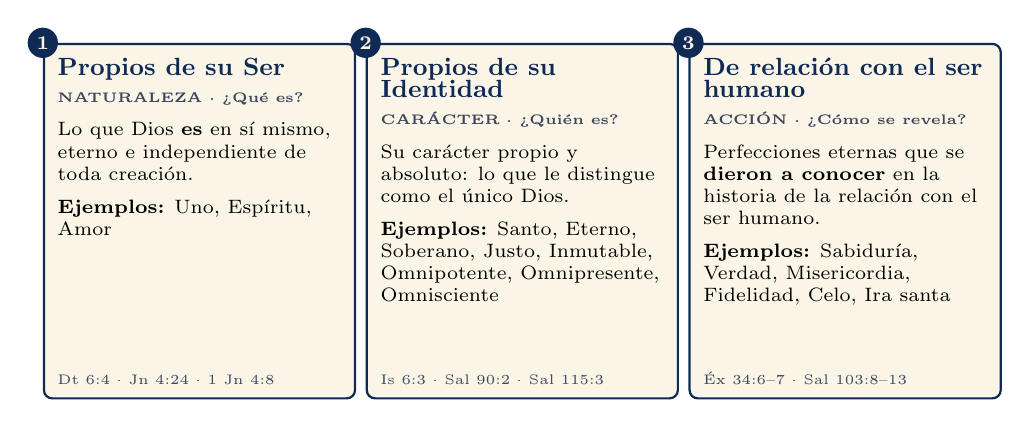
\begin{tikzpicture}
 \foreach \x/\n/\t/\k/\d/\e/\r in {
   0/1/{Propios de su Ser}/{NATURALEZA · ¿Qué es?}/{Lo que Dios \textbf{es} en sí mismo, eterno e independiente de toda creación.}/{Uno, Espíritu, Amor}/{Dt 6:4 · Jn 4:24 · 1 Jn 4:8},
   4.1/2/{Propios de su Identidad}/{CARÁCTER · ¿Quién es?}/{Su carácter propio y absoluto: lo que le distingue como el único Dios.}/{Santo, Eterno, Soberano, Justo, Inmutable, Omnipotente, Omnipresente, Omnisciente}/{Is 6:3 · Sal 90:2 · Sal 115:3},
   8.2/3/{De relación con el ser humano}/{ACCIÓN · ¿Cómo se revela?}/{Perfecciones eternas que se \textbf{dieron a conocer} en la historia de la relación con el ser humano.}/{Sabiduría, Verdad, Misericordia, Fidelidad, Celo, Ira santa}/{Éx 34:6–7 · Sal 103:8–13}}{
  \node[caja,anchor=north] (b\n) at (\x,0) {\parbox[t][4.15cm][t]{3.6cm}{\RaggedRight
    {\small\textbf{\textcolor{azulp}{\t}}}\\[2pt]{\tiny\bfseries\color{grisaz}\k}\\[4pt]\scriptsize \d\\[4pt]\textbf{Ejemplos:} \e\par\vfill{\tiny\color{grisaz}\r}}};
  \node[circle,fill=azulp,text=azulcl,font=\scriptsize\bfseries,inner sep=1.6pt] at (b\n.north west) {\n};}
\end{tikzpicture}
\end{frame}

\clasif{p_tierra.jpg}{Atributos de su Ser}{NATURALEZA}
 {Lo que Dios \emph{es} en su ser interior, eterno e independiente de la creación.}
 {ser eterno y autosuficiente; no condicionado por nada externo; esencia inmutable.}
 {Uno, Espíritu, Amor.}
 {Origen: ser puro; no dependen de nada externo.}
 {Dt 6:4 · Is 45:5 · Jn 4:24 · 1 Jn 1:5 · 1 Jn 4:8}

\clasif{p_cielo.jpg}{Atributos de su Identidad}{CARÁCTER}
 {Cómo es Dios en su esencia eterna; su carácter propio y absoluto, sus eternas perfecciones.}
 {identidad eterna de Dios; expresan lo que Dios \emph{es} en sí mismo.}
 {Santo, Eterno, Soberano, Justo, Inmutable, Omnipotente, Omnipresente, Omnisciente.}
 {Origen: identidad eterna.}
 {Sal 115:3 · Ap 4:11 · Jn 5:26 · Sal 119:68}

\clasif{p_tierra_america.jpg}{Atributos de relación}{ACCIÓN}
 {Cómo Dios se comporta hacia la creación y responde al pecado.}
 {dimensión relacional; manifestación histórica del carácter divino. Son eternos, pero se fueron revelando en la relación con el ser humano.}
 {Sabiduría, Verdad, Misericordia, Fidelidad, Celo, Ira santa, Bondad, Paciencia, Gracia.}
 {Relación: se manifiestan al relacionarse con las criaturas y ante el pecado.}
 {Éx 34:6–7 · Sal 103:8–13}

\begin{frame}{Eternos, pero revelados en la historia}
\small Todos los atributos son eternos. Los \destacar{de relación} no comenzaron a existir con el ser humano: \destacar{comenzaron a verse} en su trato con él.
\vspace{6pt}

\centering
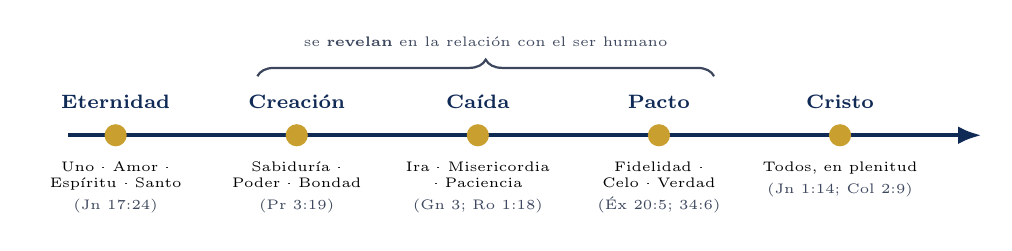
\begin{tikzpicture}
 \draw[line width=1.6pt,azulp,-{Latex[length=3mm]}] (0,0) -- (11.6,0);
 \foreach \x/\t/\a/\r in {0.6/{Eternidad}/{Uno · Amor · Espíritu · Santo}/{Jn 17:24},
                         2.9/{Creación}/{Sabiduría · Poder · Bondad}/{Pr 3:19},
                         5.2/{Caída}/{Ira · Misericordia · Paciencia}/{Gn 3; Ro 1:18},
                         7.5/{Pacto}/{Fidelidad · Celo · Verdad}/{Éx 20:5; 34:6},
                         9.8/{Cristo}/{Todos, en plenitud}/{Jn 1:14; Col 2:9}}{
  \fill[celeste] (\x,0) circle (4pt);
  \node[above=6pt,font=\scriptsize\bfseries,text=azulp] at (\x,0) {\t};
  \node[below=6pt,text width=2.0cm,align=center,font=\tiny] at (\x,0) {\a\\[2pt]{\color{grisaz}(\r)}};}
 \draw[decorate,decoration={brace,amplitude=6pt},line width=0.8pt,grisaz] (2.4,0.75) -- (8.2,0.75)
   node[midway,above=7pt,font=\tiny]{se \textbf{revelan} en la relación con el ser humano};
\end{tikzpicture}
\vspace{6pt}

\raggedright
{\footnotesize\color{grisaz}\textbf{Precisión:} la ira y la misericordia son perfecciones eternas (la santidad y el amor de Dios); lo que es histórico es su \emph{manifestación} ante el pecado y la miseria.}
\end{frame}

\begin{frame}{Comunicables e incomunicables}
\begin{columns}[t,onlytextwidth]
\begin{column}{0.48\textwidth}
\begin{tcolorbox}[colback=azulp,colframe=azulp,coltext=white,boxrule=0pt,arc=3pt,fontupper=\small]
\textbf{Incomunicables (no transferibles)}\\[3pt] Solo Dios los posee.\\[3pt]
{\footnotesize Uno · Eterno · Inmutable · Omnipresente · Omnipotente · Omnisciente}
\end{tcolorbox}
\begin{cita}Porque yo soy Dios, y no hay otro Dios, y nada hay semejante a mí.\fuente{(Is 46:9)}\end{cita}
\end{column}
\begin{column}{0.48\textwidth}
\begin{tcolorbox}[colback=azulcl,colframe=azulp,boxrule=0.8pt,arc=3pt,fontupper=\small]
\textbf{Comunicables (transferibles)}\\[3pt] Dios los refleja, en forma limitada, en el ser humano.\\[3pt]
{\footnotesize Amor · Santidad · Justicia · Sabiduría · Verdad · Misericordia · Fidelidad · Bondad · Paciencia · Gracia}
\end{tcolorbox}
\begin{cita}Y creó Dios al hombre a su imagen, a imagen de Dios lo creó.\fuente{(Gn 1:27)}\end{cita}
\end{column}
\end{columns}
\end{frame}

\begin{frame}{Las dos clasificaciones juntas}
\centering
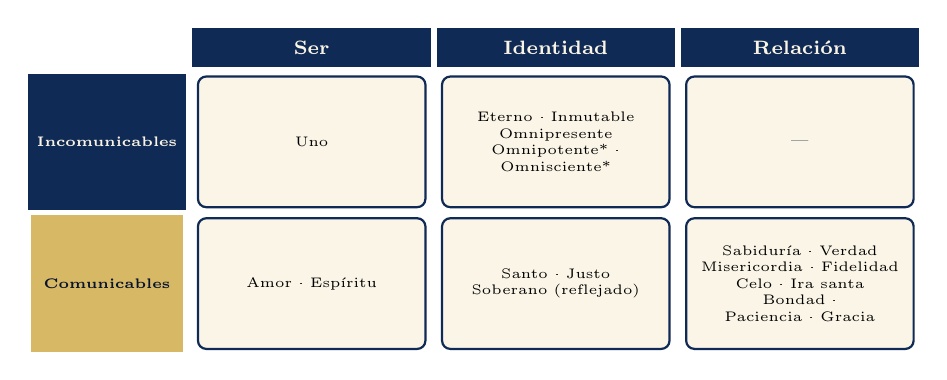
\begin{tikzpicture}[font=\scriptsize]
 \def\cw{3.1} \def\rh{1.8}
 \foreach \c/\t in {0/{Ser},1/{Identidad},2/{Relación}}{
   \node[fill=azulp,text=azulcl,font=\scriptsize\bfseries,minimum width=\cw cm-2pt,minimum height=0.5cm] at (2.1+\c*\cw+\cw/2,0.3) {\t};}
 \node[fill=azulp,text=azulcl,font=\tiny\bfseries,minimum width=2.0cm-2pt,minimum height=\rh cm-2pt,align=center] at (1.05,-\rh/2) {Incomunicables};
 \node[fill=celeste!75,text=azulo,font=\tiny\bfseries,minimum width=2.0cm-2pt,minimum height=\rh cm-2pt,align=center] at (1.05,-\rh*1.5) {Comunicables};
 \foreach \c/\r/\t in {0/0/{Uno},
                       1/0/{Eterno · Inmutable\\Omnipresente\\Omnipotente* · Omnisciente*},
                       2/0/{\color{grisaz}—},
                       0/1/{Amor · Espíritu},
                       1/1/{Santo · Justo\\Soberano (reflejado)},
                       2/1/{Sabiduría · Verdad\\Misericordia · Fidelidad\\Celo · Ira santa\\Bondad · Paciencia · Gracia}}{
   \node[caja,text width=\cw cm-16pt,minimum height=\rh cm-4pt,align=center,font=\tiny] at (2.1+\c*\cw+\cw/2,-\rh*\r-\rh/2) {\t};}
\end{tikzpicture}
\vspace{6pt}

\raggedright
{\footnotesize\color{grisaz}* Lo infinito no se comunica, pero sí su reflejo finito: poder y conocimiento. Espíritu se ubica entre los comunicables siguiendo a Berkhof (1938): el ser humano recibe espíritu (Gn 2:7), no la espiritualidad infinita de Dios.}
\end{frame}

% =====================================================================
% =====================================================================
\begin{frame}{Todos los atributos, en Cristo}
\begin{cita}Porque en él habita corporalmente toda la plenitud de la Deidad.\fuente{(Col 2:9)}\end{cita}
\begin{cita}El que me ha visto a mí, ha visto al Padre.\fuente{(Jn 14:9)}\end{cita}
\vspace{4pt}
\small Cada atributo de esta serie terminará con un apartado: \destacar{cómo se reflejó en Cristo}. La serie concluirá mostrando que la gloria de Dios es la comunión de todos sus atributos, y que esa plenitud habita en Él.
\end{frame}

\begin{frame}{Todos los atributos convergen en Él}
\centering
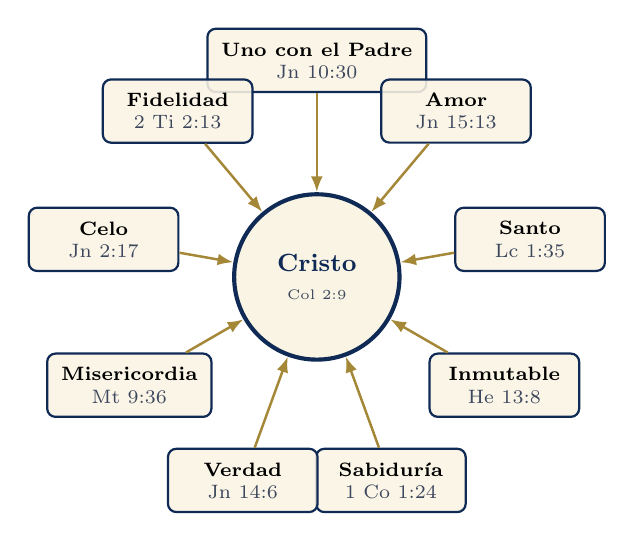
\begin{tikzpicture}[font=\tiny]
 \node[circle,draw=azulp,line width=1.5pt,fill=azulcl,minimum size=2.1cm,align=center,font=\small\bfseries,text=azulp] (c) at (0,0) {Cristo\\[-1pt]{\tiny\mdseries\color{grisaz}Col 2:9}};
 \foreach \a/\t/\r in {90/{Uno con el Padre}/{Jn 10:30},
                       50/{Amor}/{Jn 15:13},
                       10/{Santo}/{Lc 1:35},
                       -30/{Inmutable}/{He 13:8},
                       -70/{Sabiduría}/{1 Co 1:24},
                       -110/{Verdad}/{Jn 14:6},
                       -150/{Misericordia}/{Mt 9:36},
                       170/{Celo}/{Jn 2:17},
                       130/{Fidelidad}/{2 Ti 2:13}}{
   \node[caja,align=center,minimum width=1.9cm] (n\a) at (\a:2.75cm) {\textbf{\t}\\{\color{grisaz}\r}};
   \draw[-{Latex[length=2mm]},celeste!80!azulp,line width=0.9pt] (n\a) -- (c);}
\end{tikzpicture}
\vspace{2pt}

{\footnotesize Juan 1:14 retoma Éx 34:6: el Verbo hecho carne vino “lleno de \destacar{gracia} y de \destacar{verdad}”.}
\end{frame}

\begin{frame}{Cómo se estudiará cada atributo}
\small Cada capítulo del libro y cada presentación seguirán la misma ruta:
\vspace{4pt}

\centering
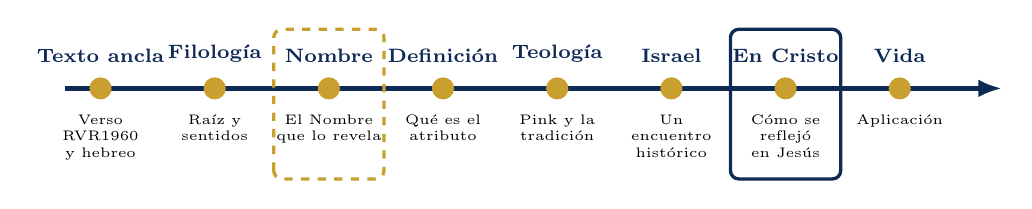
\begin{tikzpicture}
 \draw[line width=1.6pt,azulp,-{Latex[length=3mm]}] (0,0) -- (11.9,0);
 \foreach \x/\t/\d in {0.45/{Texto ancla}/{Verso RVR1960 y hebreo},
                      1.9/{Filología}/{Raíz y sentidos},
                      3.35/{Nombre}/{El Nombre que lo revela},
                      4.8/{Definición}/{Qué es el atributo},
                      6.25/{Teología}/{Pink y la tradición},
                      7.7/{Israel}/{Un encuentro histórico},
                      9.15/{En Cristo}/{Cómo se reflejó en Jesús},
                      10.6/{Vida}/{Aplicación}}{
  \fill[celeste] (\x,0) circle (4pt);
  \node[above=6pt,font=\scriptsize\bfseries,text=azulp] at (\x,0) {\t};
  \node[below=6pt,text width=1.35cm,align=center,font=\tiny] at (\x,0) {\d};}
 \draw[azulp,line width=1.2pt,rounded corners=3pt] (8.45,-1.15) rectangle (9.85,0.75);
 \draw[celeste,line width=1.2pt,rounded corners=3pt,dashed] (2.65,-1.15) rectangle (4.05,0.75);
\end{tikzpicture}
\vspace{8pt}

\raggedright
{\footnotesize\color{grisaz}El apartado \textbf{“En Cristo”} es obligatorio en todos los capítulos: la serie termina mostrando que la \textbf{gloria de Dios es la comunión de todos sus atributos}, y que esa plenitud habita en Cristo (Col 1:19).}
\end{frame}

% =====================================================================
\section{Los nombres}
% =====================================================================
\providecommand{\precision}[1]{{\footnotesize\color{grisaz}\textbf{Precisión:} #1}}

\begin{frame}{``Según mis obras soy llamado''}
\begin{columns}[c,onlytextwidth]
\begin{column}{0.48\textwidth}
\small Si el Nombre es la colección de sus atributos, \destacar{cada nombre de Dios revela algo de lo que él es}. No todos los atributos tienen un nombre propio, pero la gran mayoría está ligada a un nombre, un título o una declaración con el Nombre.\par\medskip
\begin{center}\heb{שמי אתה מבקש לידע לפי מעשי אני נקרא}\end{center}
\footnotesize ``¿Mi nombre quieres saber? Según mis obras soy llamado'' (\emph{Shemot Rabá} 3:6, sobre Éx 3:13).\par\smallskip
\precision{lectura rabínica (R. Abbá bar Memel), no etimología.}
\end{column}
\begin{column}{0.50\textwidth}
\centering
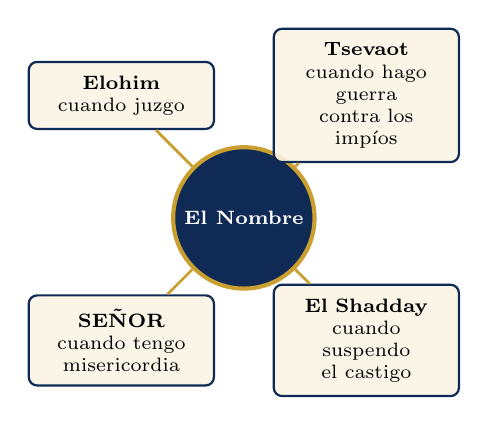
\begin{tikzpicture}[font=\scriptsize]
 \node[circle,draw=celeste,line width=1.5pt,fill=azulp,text=white,minimum size=1.6cm,align=center,font=\scriptsize\bfseries] (d) at (0,0) {El Nombre};
 \foreach \a/\n/\o in {135/Elohim/{cuando juzgo},45/Tsevaot/{cuando hago guerra\\contra los impíos},-45/{El Shadday}/{cuando suspendo\\el castigo},-135/\SENOR{}/{cuando tengo\\misericordia}}{
   \node[caja,text width=2.0cm,align=center] (n\a) at (\a:2.2cm) {\textbf{\n}\\\o};
   \draw[celeste,line width=1pt] (d) -- (n\a);}
\end{tikzpicture}
\end{column}
\end{columns}
\end{frame}

\begin{frame}{``YO SOY EL QUE SOY''}
\begin{columns}[c,onlytextwidth]
\begin{column}{0.50\textwidth}
\begin{cita}Y respondió Dios a Moisés: YO SOY EL QUE SOY. Y dijo: Así dirás a los hijos de Israel: YO SOY me envió a vosotros.\fuente{(Éx 3:14, RVR1960)}\end{cita}
\begin{center}\heb{אֶהְיֶה אֲשֶׁר אֶהְיֶה}\end{center}
\scriptsize ``Este es mi nombre para siempre; con él se me recordará por todos los siglos'' (Éx 3:15).\par\smallskip
\small Este Nombre habla ante todo de la \destacar{eternidad}: Dios simplemente es. ``Antes que Abraham fuese, yo soy'' (Jn 8:58); ``el que es y que era y que ha de venir'' (Ap 1:8).
\end{column}
\begin{column}{0.48\textwidth}\scriptsize
\renewcommand{\arraystretch}{1.2}
\begin{tabular}{@{}>{\RaggedRight\arraybackslash}p{2.0cm}>{\RaggedRight\arraybackslash}p{3.7cm}@{}}
\toprule
\textbf{Término} & \textbf{Sentido} \\ \midrule
\heb{אֶהְיֶה} \emph{ehyeh} & imperfecto de \heb{היה}: ``soy / seré''; acción no terminada. \\
\heb{יְהוָה} YHWH & el Nombre propio (v.~15): Dios dice ``Yo soy'', Israel dice ``Él es''. Etimología discutida (HALOT). \\
\heb{לְעֹלָם} \emph{le'olam} & ``para siempre''. \\
\grc{ἐγώ εἰμι ὁ ὤν} & LXX: ``Yo soy el que es''. \\
\bottomrule
\end{tabular}\par\medskip
\precision{Rashi (con Berajot 9b): ``estaré con ellos en esta angustia''. La lectura judía subraya la presencia fiel; la LXX y Jn 8:58, el ser eterno. No se excluyen.}
\end{column}
\end{columns}
\end{frame}

\begin{frame}{Mapa de los nombres (I): Ser e Identidad}
\tiny\renewcommand{\arraystretch}{1.1}
\begin{tabular}{@{}>{\RaggedRight\arraybackslash}p{1.6cm}>{\RaggedRight\arraybackslash}p{3.9cm}>{\RaggedRight\arraybackslash}p{3.1cm}>{\RaggedRight\arraybackslash}p{1.9cm}@{}}
\toprule
\textbf{Atributo} & \textbf{Nombre o declaración} & \textbf{Original} & \textbf{Texto} \\ \midrule
Preexistente & ``Yo soy el primero, y yo soy el postrero'' & \heb{אֲנִי רִאשׁוֹן וַאֲנִי אַחֲרוֹן} & Is 44:6; Ap 1:8 \\
Uno & ``El \SENOR{} uno es''; ``uno su nombre'' & \heb{יְהוָה אֶחָד} & Dt 6:4; Zac 14:9 \\
Amor & ``El Dios de paz y de amor'' & \grc{ὁ θεὸς τῆς ἀγάπης} & 2~Co 13:11 \\
Espíritu & ``Dios de los espíritus de toda carne'' & \heb{אֵל אֱלֹהֵי הָרוּחֹת} & Nm 16:22 \\ \midrule
Santo & ``El Santo de Israel''; ``su nombre es el Santo'' & \heb{קְדוֹשׁ יִשְׂרָאֵל} & Is 41:14; 57:15 \\
Eterno & ``YO SOY EL QUE SOY''; ``Dios eterno'' & \heb{אֶהְיֶה}; \heb{אֵל עוֹלָם} & Éx 3:14; Gn 21:33 \\
Soberano & ``Dios Altísimo''; ``el solo Soberano'' & \heb{אֵל עֶלְיוֹן}; \grc{μόνος δυνάστης} & Gn 14:19; 1~Ti 6:15 \\
Justo & ``\SENOR{}, justicia nuestra'' & \heb{יְהוָה צִדְקֵנוּ} & Jer 23:6 \\
Inmutable & ``Yo \SENOR{} no cambio''; ``la Roca'' & \heb{לֹא שָׁנִיתִי}; \heb{הַצּוּר} & Mal 3:6; Dt 32:4 \\
Omnipotente & ``Dios Todopoderoso''; ``\SENOR{} de los ejércitos'' & \heb{אֵל שַׁדַּי}; \heb{יְהוָה צְבָאוֹת} & Gn 17:1; Is 6:3 \\
Omnipresente & ``\SENOR{}-sama''; ``Emanuel'' & \heb{יְהוָה שָׁמָּה}; \heb{עִמָּנוּאֵל} & Ez 48:35; Is 7:14 \\
Omnisciente & ``Dios que ve''; ``Dios de todo saber'' & \heb{אֵל רֳאִי}; \heb{אֵל דֵּעוֹת} & Gn 16:13; 1~S 2:3 \\
\bottomrule
\end{tabular}
\end{frame}

\begin{frame}{Mapa de los nombres (II): Relación}
\tiny\renewcommand{\arraystretch}{1.1}
\begin{tabular}{@{}>{\RaggedRight\arraybackslash}p{1.6cm}>{\RaggedRight\arraybackslash}p{3.9cm}>{\RaggedRight\arraybackslash}p{3.1cm}>{\RaggedRight\arraybackslash}p{1.9cm}@{}}
\toprule
\textbf{Atributo} & \textbf{Nombre o declaración} & \textbf{Original} & \textbf{Texto} \\ \midrule
Sabiduría & ``Admirable, Consejero''; ``el único y sabio Dios'' & \heb{פֶּלֶא יוֹעֵץ}; \grc{μόνῳ σοφῷ θεῷ} & Is 9:6; Ro 16:27 \\
Verdadero & ``Dios de verdad''; ``el Dios del Amén'' & \heb{אֵל אֱמֶת}; \heb{אֱלֹהֵי אָמֵן} & Sal 31:5; Is 65:16 \\
Misericordioso & ``Dios misericordioso''; ``Padre de misericordias'' & \heb{אֵל רַחוּם} & Dt 4:31; 2~Co 1:3 \\
Fiel & ``Dios fiel'' & \heb{הָאֵל הַנֶּאֱמָן} & Dt 7:9; 1~Co 1:9 \\
Celo & ``Cuyo nombre es Celoso'' & \heb{קַנָּא שְׁמוֹ} & Éx 34:14 \\
Ira santa & ``Dios de las venganzas'' & \heb{אֵל נְקָמוֹת} & Sal 94:1; Nah 1:2 \\
Bondad & ``\SENOR{} proveerá''; ``es bueno el \SENOR{}'' & \heb{יְהוָה יִרְאֶה}; \heb{טוֹב יְהוָה} & Gn 22:14; Sal 34:8 \\
Paciencia & ``Tardo para la ira''; ``el Dios de la paciencia'' & \heb{אֶרֶךְ אַפַּיִם}; \grc{ὑπομονή} & Éx 34:6; Ro 15:5 \\
Gracia & ``Piadoso''; ``el Dios de toda gracia'' & \heb{חַנּוּן}; \grc{πάσης χάριτος} & Éx 34:6; 1~P 5:10 \\
\bottomrule
\end{tabular}\par\smallskip
\precision{no todos son nombres propios: algunos son títulos, otros declaraciones con el Nombre (Mal 3:6) o nombres de lugares (Gn 22:14; Ez 48:35). Los sabios agregaron \emph{HaQadosh Barukh Hu}, \emph{HaRajamán}, \emph{Ribbonó shel olam} y \emph{HaMaqom}, ``el Lugar'' (\emph{Bereshit Rabá} 68:9).}
\end{frame}

\begin{frame}{El Nombre que es sobre todo nombre}
\begin{columns}[c,onlytextwidth]
\begin{column}{0.50\textwidth}
\begin{cita}Por mí mismo hice juramento, de mi boca salió palabra en justicia, y no será revocada: Que a mí se doblará toda rodilla, y jurará toda lengua.\fuente{(Is 45:23, RVR1960)}\end{cita}
\begin{cita}Por lo cual Dios también le exaltó hasta lo sumo, y le dio un nombre que es sobre todo nombre, para que en el nombre de Jesús se doble toda rodilla de los que están en los cielos, y en la tierra, y debajo de la tierra; y toda lengua confiese que Jesucristo es el Señor, para gloria de Dios Padre.\fuente{(Flp 2:9--11, RVR1960)}\end{cita}
\end{column}
\begin{column}{0.48\textwidth}\small
\begin{itemize}
\item Pablo aplica a Jesús un texto en que el \SENOR{} reclama para sí solo la adoración de toda la tierra.
\item \grc{κύριος}, ``Señor'', es la palabra con que la Septuaginta traduce \heb{יְהוָה}.
\item Cada nombre del mapa \destacar{converge en ese Nombre}: en él habita toda la plenitud de la Deidad (Col 2:9).
\end{itemize}
\end{column}
\end{columns}
\end{frame}

% =====================================================================
\section{Nuestra gloria}
% =====================================================================
\begin{frame}{Nuestra gloria}
\tiny
\begin{tabular}{@{}P{1.2cm} P{4.9cm} P{4.9cm}@{}}
\toprule
\textbf{Cita bíblica} & \textbf{Reina-Valera 1960 (RVR60)} & \textbf{Nueva Versión Internacional (NVI)} \\ \midrule
Sal 44:8 & En Dios nos gloriaremos todo el tiempo, y para siempre alabaremos tu nombre. & Por siempre nos gloriaremos en Dios; ¡por siempre alabaremos tu nombre! \\
Is 41:16 & …pero tú te regocijarás en el \SENOR, te gloriarás en el Santo de Israel. & …Pero tú te alegrarás en el Señor; te gloriarás en el Santo de Israel. \\
Is 45:25 & En el \SENOR{} será justificada y se gloriará toda la descendencia de Israel. & Pero toda la descendencia de Israel será justificada por el Señor, y en él se gloriará. \\
Ro 5:11 & Y no sólo esto, sino que también nos gloriamos en Dios por el Señor nuestro Jesucristo, por quien hemos recibido ahora la reconciliación. & Y no solo esto, sino que también nos regocijamos en Dios por nuestro Señor Jesucristo, pues gracias a él ya hemos recibido la reconciliación. \\
2 Co 10:17 & Mas el que se gloría, gloríese en el Señor. & «Si alguien ha de gloriarse, que se gloríe en el Señor». \\ \bottomrule
\end{tabular}
\end{frame}

% =====================================================================
\section{Ejemplo revelador}
\begin{frame}[plain]
\begin{tikzpicture}[remember picture,overlay]
 \fill[black] (current page.south west) rectangle (current page.north east);
 \node[anchor=west,inner sep=0] at (current page.west) {
\includegraphics[height=\paperheight,width=0.62\paperwidth]{fuego.jpg}};
 \node[anchor=east,inner sep=0] at (current page.east) {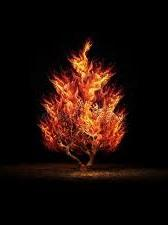
\includegraphics[height=\paperheight,width=0.42\paperwidth]{zarza.jpg}};
 \fill[azulo,opacity=0.80] ([yshift=-0.16\paperheight]current page.west) rectangle ([yshift=0.16\paperheight]current page.east);
 \node[text=white,font=\LARGE\bfseries,align=center] at ([yshift=0.04\paperheight]current page.center) {Cuando Dios se revela, no solo habla: transforma.};
 \node[text=celeste!70!white,font=\small\itshape,align=center] at ([yshift=-0.07\paperheight]current page.center) {“YO SOY EL QUE SOY” (Éx 3:14)};
\end{tikzpicture}
\end{frame}

% =====================================================================
\section{Conclusiones}
% =====================================================================
\begin{frame}{Conclusiones}
\fotolado{p_tierra_final.jpg}{}
\begin{columns}[c,onlytextwidth]
\begin{column}{0.57\textwidth}
\small
\begin{enumerate}
\item Entender a Dios no significa abarcarlo con una mente finita, sino reconocerlo según lo que Él mismo ha revelado de su ser.\par\vspace{6pt}
\item Conocer a Dios es reconocer quién es Él y cómo actúa, especialmente en sus atributos.\par\vspace{6pt}
\item El conocimiento verdadero de Dios transforma la vida, porque al conocerlo, el hombre se alinea con su voluntad.
\end{enumerate}
\end{column}
\begin{column}{0.41\textwidth}\end{column}
\end{columns}
\end{frame}

\begin{frame}{Referencias}
\scriptsize
\refapa{Marshall, B. J., Armstrong, J. A., McGechie, D. B., \& Glancy, R. J. (1985). Attempt to fulfil Koch's postulates for pyloric \emph{Campylobacter}. \emph{Medical Journal of Australia, 142}(8), 436–439.}
\refapa{Pink, A. W. (2020). \emph{Los atributos de Dios} (E. Rodríguez Cruz, Trad.). Chapel Library. (Obra original publicada en 1930)}
\refapa{\emph{Santa Biblia: Nueva Versión Internacional}. (1999). Sociedad Bíblica Internacional.}
\refapa{\emph{Santa Biblia: Reina-Valera 1960}. (1960). Sociedades Bíblicas en América Latina.}
\vspace{6pt}
{\footnotesize\color{grisaz}Donde la RVR1960 dice “Jehová”, se escribe \SENOR.}
\end{frame}

\end{document}
